% Build from this directory with latexmk -pdf territory_control_report.tex.
% Official style: https://neurips.cc/Conferences/2023/PaperInformation/StyleFiles
\documentclass{article}

\usepackage[preprint]{neurips_2023}
\usepackage[T1]{fontenc}
\usepackage[utf8]{inputenc}
\usepackage{amsmath}
\usepackage{booktabs}
\usepackage{float}
\usepackage{tabularx}
\usepackage{microtype}
\usepackage{tikz}
\usetikzlibrary{arrows.meta}
\usepackage{url}
\usepackage[hidelinks]{hyperref}
\hypersetup{
  pdftitle={Action Commitments and Proposals in Team-Based Territory Control},
  pdfauthor={Hohyung Lee, Jongbin Kim, Dohyung Kim},
  pdfsubject={CS30707 course project report draft}
}

% Set the first-page notice for the course draft using the official layout.
\makeatletter
\renewcommand{\@noticestring}{CS30707 course project report draft.}
\makeatother

\title{Action Commitments and Proposals in Team-Based Territory Control}

\author{
  Hohyung Lee \qquad Jongbin Kim \qquad Dohyung Kim \\
  KAIST \\
  CS30707, Team 1
}

\begin{document}

\maketitle

\begin{abstract}
We introduce Territory Control, a three-versus-three benchmark that measures how seeing teammates' action proposals affects decisions at execution and how receiver-to-sender gradients affect the policy learned during training. Independent decisions, fixed-order commitments, and revisable proposals all use the same simultaneous transition. In a shared-reward PPO pilot, we replay the same boards and opposing actions to compare cover on 3,274 matched opportunities. Revealing proposals to the checkpoint trained with receiver gradients blocked increases successful cover from 449 to 517. With proposals visible for both sharing policies, the model trained with gradients blocked records 275 more successful covers. A gap of 228 successes remains with teammate proposals masked for both policies. The policy trained with teammate proposals masked achieves the highest match score, 26.95\% across 384 games.
\end{abstract}

\section{Introduction}

Teammate communication acts at two stages. At execution, seeing an ally's proposed action can change which tile an agent defends. During learning, gradients through the proposal channel can change the policy that makes those decisions. We study both effects under a shared territory objective, where agents learn who should defend, advance, or yield. The reward-is-enough hypothesis and the cooperative strategies observed in multi-agent hide-and-seek motivate studying these behaviors under team-level incentives \citep{silver2021reward,baker2020autocurricula}.

Territory Control makes these effects measurable under common game rules. The decision protocol determines whether agents act independently, see earlier teammates' committed actions in a fixed order, or exchange tentative proposals before deciding again. All six final actions resolve together after collection. Each actor can see the entire board, and the protocol determines its access to teammate choices for the current tick. Individual capture credit and shared team rewards are configurable for each protocol.

In the shared-reward PPO pilot, we test proposal use by toggling teammate visibility for the same checkpoint and first-round proposals. To test the training effect, we train with teammate proposals visible and vary whether the receiver loss can backpropagate through the sender's proposal. Both conditions use the same discrete forward channel. Replaying the same positions with the same opposing actions lets us compare both effects on the same cover opportunities. Full matches track score and final territory against multiple opponents, including bots held out from training. Independent-policy runs establish baseline strengths for the planned matched comparison.

\clearpage
\section{Related work}
\label{sec:related}

\paragraph{Multi-agent benchmarks.}
Pommerman offers a two-versus-two grid game with a radio variant that allows discrete messages between teammates \citep{resnick2018pommerman}. Territory Paint Wars uses simultaneous tile competition between two players to diagnose failures of PPO self-play \citep{singh2026paintwars}. Melting Pot 2.0 evaluates policies alongside unfamiliar co-players across environments that include Territory \citep{agapiou2022meltingpot}. MARL-BattleGrounds pairs team matches with short tactical endgame tests on held-out positions \citep{hawili2026battlegrounds}. Territory Control keeps the transition rules fixed across protocols and varies whether agents can observe teammates' committed actions or tentative proposals for the current tick. Replays let us measure the effect of that information on a common set of tactical opportunities.

\paragraph{Sequential decision making.}
\citet{ding2024seqcomm} propose SeqComm, which assigns decision priority by exchanging encoded observations and evaluating predicted intentions. Agents then pass committed actions to teammates that decide later, and the environment executes the resulting actions simultaneously. Our protocol fixes the within-team order by slot and exposes the prefix of committed actions on a frozen board. This makes it possible to mask the prefix while holding decision order fixed. The Multi-Agent Transformer also generates actions in sequence, using one encoder-decoder over the agents' observations and an autoregressive joint-action decoder \citep{wen2022mat}. In our protocol each actor call takes its own observation and the commits the environment has made visible to that slot.

\paragraph{Intention sharing and message gradients.}
\citet{kim2021intention} use learned dynamics and models of teammates to generate and communicate compressed future trajectories. In our two-round protocol, each agent sends one of nine actions for the \emph{current} tick, receives the team's first-round proposals, and can revise its own action before execution. Multi-task Communication Skills (MCS) couples a learned message representation to the sender's executed actions through a prediction objective \citep{zhu2026mcs}. We use this objective to predict a sender's second-round action from its first-round action index. DIAL backpropagates through a real-valued channel during centralized training and quantizes messages at execution \citep{foerster2016dial}. Our receiver sees the recorded discrete proposal in the forward pass. A straight-through estimator lets us vary whether its policy gradient reaches the sender's proposal distribution while retaining the same proposal format.

\paragraph{Evaluating communication and cooperation.}
SMACv2 introduced procedurally generated scenarios after showing that policies conditioned only on time could win some SMAC games \citep{ellis2023smacv2}. Coordination diagnostics can also reveal differences in interference and joint task completion between policies with similar returns \citep{cardei2026coordination}. \citet{lowe2019pitfalls} distinguish \emph{positive signaling}, in which a message carries information about a sender, from \emph{positive listening}, in which that message changes a receiver's behavior. We test listening with a fixed checkpoint and first-round proposals and count the consequences for cover and movement. Full matches capture how these decisions affect the positions each policy goes on to visit.


\section{Methods}
\label{sec:methods}

\paragraph{Controlled territory game.}
Two teams of three start with equal territory. Each agent can wait, move in one of four directions, or attack an adjacent tile. Teams sum attacks on each tile, and ties preserve ownership. The engine resolves attacks before movement, with a one-tick attack cooldown. Agents on enemy tiles die, moves to the same destination fail, and a teammate can enter a tile vacated by another agent. Eligible agents can respawn on vacant friendly tiles at the end of the tick. A match ends at the horizon or when one team has neither survivors nor territory. Final territory determines the result.

\paragraph{Decision protocols.}
The team-relative observation \(o_i\) includes the entire board, agent status, slot identity, and legal-action mask. Figure~\ref{fig:protocols} varies the information available before the same joint transition. Independent actors act from \(o_i\). In fixed order, slot \(i\) also sees earlier slots' committed actions \(a_1,\ldots,a_{i-1}\). In proposal sharing, all slots first choose a legal action index \(m_i\) and then choose final actions from the frozen broadcast. During collection, each actor can receive actions only from its own team.

\begin{figure}[tb]
  \centering
  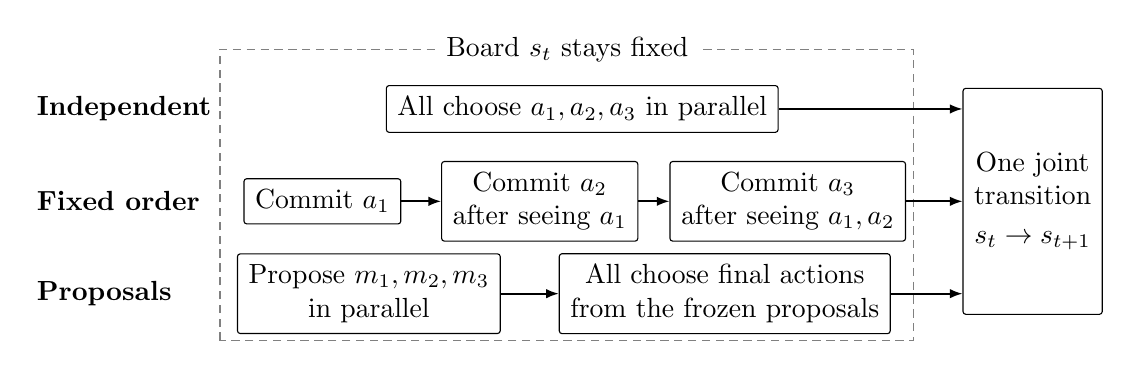
\begin{tikzpicture}[
    x=1cm, y=1.15cm,
    box/.style={draw, rounded corners=1pt, inner xsep=4pt, inner ysep=4pt, align=center},
    flow/.style={-{Latex[length=1.6mm]}, semithick},
    row label/.style={anchor=west, font=\bfseries}
  ]
    \draw[gray, densely dashed] (2.45,-0.46) rectangle (11.26,2.76);
    \node[fill=white, inner xsep=4pt] at (6.86,2.76) {Board \(s_t\) stays fixed};
    \node[row label] at (0,2.10) {Independent};
    \node[row label] at (0,1.08) {Fixed order};
    \node[row label] at (0,0.06) {Proposals};

    \node[box] (independent) at (7.05,2.10) {All choose \(a_1,a_2,a_3\) in parallel};
    \node[box] (first) at (3.75,1.08) {Commit \(a_1\)};
    \node[box] (second) at (6.51,1.08) {Commit \(a_2\)\\after seeing \(a_1\)};
    \node[box] (third) at (9.66,1.08) {Commit \(a_3\)\\after seeing \(a_1,a_2\)};
    \node[box] (propose) at (4.34,0.06) {Propose \(m_1,m_2,m_3\)\\in parallel};
    \node[box] (revise) at (8.86,0.06) {All choose final actions\\from the frozen proposals};

    \node[box, minimum height=2.87cm, minimum width=1.67cm] (transition) at (12.77,1.08)
      {One joint\\transition\\[2pt]\(s_t\to s_{t+1}\)};
    \draw[flow] (first.east) -- (second.west);
    \draw[flow] (second.east) -- (third.west);
    \draw[flow] (propose.east) -- (revise.west);
    \draw[flow] (independent.east) -- (transition.west |- independent.east);
    \draw[flow] (third.east) -- (transition.west);
    \draw[flow] (revise.east) -- (transition.west |- revise.east);
  \end{tikzpicture}
  \caption{Information available within one tick. The diagram shows one team. The engine collects both teams' final actions before advancing the game.}
  \label{fig:protocols}
\end{figure}

\paragraph{Actor and critic design.}
Feedback PPO shares a CNN across the learning team's agents. It reads two ownership channels and six occupancy channels on an \(8\times10\) padded board. The CNN output and status features form the agent's 128-dimensional feature \(h_i\). The final-action head receives \(h_i\) and three 16-dimensional action embeddings, one per ally slot. Masked slots become zero vectors, distinct from a visible wait action. Both heads use legal-action masks, and the critic reads \(h_i\) alone. In the planned comparison, the independent and fixed-order actors use this final-action interface with an empty slot vector or a committed prefix, respectively. Proposal sharing adds the proposal head \(q_\theta\).

\paragraph{Two decisions per tick.}
Let \(b_i\) be the visible proposal slots and \(a_i\) the executed action. The two-round PPO update uses the per-agent log likelihood
\begin{equation}
  \log q_\theta(m_i\mid h_i) + \log \pi_\theta(a_i\mid h_i,b_i)
  \label{eq:logprob}
\end{equation}
to form the clipped ratio \citep{schulman2017ppo,yu2022mappo}. A separate predictor estimates the sender's final action from \(m_i\) using cross-entropy with weight \(0.1\). To test the effect of the receiver gradient, we train two variants with teammate proposals visible. With the gradient enabled, the receiver uses \(\operatorname{onehot}(m_j)+p_j-\operatorname{sg}(p_j)\), where \(p_j\) is the sender's masked proposal distribution and \(\operatorname{sg}\) stops gradients. Both variants use recorded one-hot actions in the forward computation. With the gradient stopped, the message embedding and the receiver's action head still learn. The sender's own PPO and prediction losses train the proposal head in all feedback conditions.

\begin{figure}[H]
  \centering
  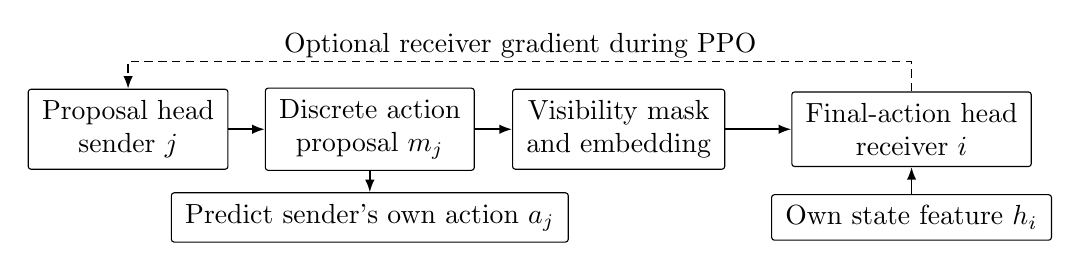
\begin{tikzpicture}[
    block/.style={draw, rounded corners=1pt, align=center, inner xsep=5pt, inner ysep=4pt},
    arrow/.style={-{Latex[length=1.6mm]}, semithick}
  ]
    \node[block] (proposal) at (1.55,0) {Proposal head\\sender \(j\)};
    \node[block] (symbol) at (4.62,0) {Discrete action\\proposal \(m_j\)};
    \node[block] (mask) at (7.78,0) {Visibility mask\\and embedding};
    \node[block] (receiver) at (11.50,0) {Final-action head\\receiver \(i\)};
    \node[block] (predict) at (4.62,-1.12) {Predict sender's own action \(a_j\)};
    \node[block] (own) at (11.50,-1.12) {Own state feature \(h_i\)};
    \draw[arrow] (proposal) -- (symbol);
    \draw[arrow] (symbol) -- (mask);
    \draw[arrow] (mask) -- (receiver);
    \draw[arrow] (symbol.south) -- (predict.north);
    \draw[arrow] (own.north) -- (receiver.south);
    \draw[arrow, densely dashed] (receiver.north) -- ++(0,0.38) -| (proposal.north);
    \node[above, inner sep=2pt] at (6.53,0.83) {Optional receiver gradient during PPO};
  \end{tikzpicture}
  \caption{Feedback PPO for one sender--receiver link. Solid arrows show the forward pass. The dashed receiver gradient is optional during training. The visibility mask changes the receiver's input, and the sender predictor is trained in all feedback conditions.}
  \label{fig:receiver}
\end{figure}

\section{Evaluation}
\label{sec:evaluation}

Table~\ref{tab:controls} specifies common settings for the planned three-protocol comparison. The world, reward, budget, and match schedule reproduce the completed feedback pilot. Full matches pair starting conditions and let trajectories evolve. Paired one-tick replays hold the board and opponent actions fixed to evaluate the same opportunities.

\begin{table}[H]
  \centering
  \caption{Controls for the matched comparison of independent, fixed-order, and proposal-sharing policies.}
  \label{tab:controls}
  \begin{tabularx}{\linewidth}{@{}>{\raggedright\arraybackslash}p{.25\linewidth}>{\raggedright\arraybackslash}X@{}}
    \toprule
    Factor & Shared setting \\
    \midrule
    Environment & Three-versus-three on \(8\times8\), frontier starts, rotation off, immediate respawn, horizon 128. \\
    Actor and critic & Same centered \(15\times15\) tilemap, status, action masks, encoder and final-head capacity, and observation-only critic. \\
    Team reward & Post-transition territory gap divided by \(8{,}192\), with terminal win/draw/loss \(+1/0/-1\). \\
    PPO budget & 100,352 ticks per seed (7, 19, 31), using \(8\times64\) ticks per update and 196 updates. \\
    PPO settings & Adam at \(3\times10^{-4}\), discount \(0.995\), GAE \(\lambda=0.95\), clip \(0.2\), four epochs and batches of 256. \\
    Training opponents & Equal mixture of \texttt{random} and \texttt{expand} by episode, with team colors alternating. \\
    Match evaluation & Final checkpoint, masked argmax, seeds 681000--681015 per opponent and both colors. \\
    \bottomrule
  \end{tabularx}
\end{table}

\begin{table}[H]
  \centering
  \caption{Common outcomes and within-state tests. Tactical rates carry both the success count and the opportunity count.}
  \label{tab:metrics}
  \begin{tabularx}{\linewidth}{@{}>{\raggedright\arraybackslash}p{.25\linewidth}>{\raggedright\arraybackslash}X@{}}
    \toprule
    Metric & What the benchmark measures \\
    \midrule
    Match outcome & Wins, draws, losses, \((W+0.5D)/N\) over \(N\) matches, and final territory gap divided by board area. \\
    Cover & An occupied ally tile is attacked and ready neighbors can match the opposing attacks. Success preserves the tile and the threatened ally through movement. \\
    Chained yield & An ally can vacate a frontier tile. Both allies move safely and the follower enters that tile. Replacing the leader's move with wait prevents the entry. \\
    Receiver action change & Fraction of replay ticks with a changed choice after masking teammate inputs to a fixed-order or proposal-sharing checkpoint. \\
    Decisive joint attack & Planned metric. Among tiles attacked by multiple allies, count cases where replacing one attack with wait changes capture or defense. \\
    \bottomrule
  \end{tabularx}
\end{table}

\paragraph{Completed evaluations.}
On \(8\times8\), we trained three feedback conditions (sharing with and without the receiver gradient, and teammate masking from training). We matched initialization by seed and evaluated 384 games per condition against \texttt{random}, \texttt{expand}, and the held-out \texttt{aggressive} and \texttt{defend}. We sampled 59,734 replay ticks from gradient-on and masked-training trajectories, taking equal numbers within each training seed, opponent, start seed, and color. This yields 3,274 common cover opportunities. We toggle visibility at fixed checkpoint and first-round proposals. A separate independent-policy pilot uses \(3\times10\) and 64 ticks to study team-size transfer and calibrate opponents.\footnote{The project repository records both experiments in \texttt{docs/feedback\_ppo\_communication.md} and \texttt{SL-RL/SL\_RL\_RESEARCH\_SUMMARY.md}.}

\paragraph{Planned matched evaluation.}
We will train all three protocols under Table~\ref{tab:controls} and compare them on a common replay pool. A two-round self-proposal-only policy controls for the extra decision stage and sender loss. Its comparison with the shared-proposal policy uses stopped receiver gradients in both conditions. To test fixed-order listening, we will hold earlier commitments and slot order fixed and mask only the receiver's view of them. The first slot serves as a control because it observes an empty prefix. We will report outcomes by opponent and training seed, and receiver effects by slot.

\section{Results}
\label{sec:results}

\begin{table}[H]
  \centering
  \caption{Feedback PPO over 384 matches and 3,274 matched cover opportunities per row.}
  \label{tab:feedback}
  \begin{tabular*}{\linewidth}{@{\extracolsep{\fill}}llrrr@{}}
    \toprule
    Training condition & Eval.\ peer proposals & Score & Full-match cover & Matched cover \\
    \midrule
    Shared, gradient on  & Visible & 19.40\% & \(194/1{,}471\)   & 242 \\
    Shared, gradient on  & Masked  & 19.53\% & \(146/1{,}427\)   & 221 \\
    Shared, gradient off & Visible & 24.61\% & \(1{,}078/2{,}459\) & 517 \\
    Shared, gradient off & Masked  & 22.79\% & \(539/1{,}831\)   & 449 \\
    Masked from training & Masked  & 26.95\% & \(1{,}665/3{,}703\) & 1{,}020 \\
    \bottomrule
  \end{tabular*}
\end{table}

\paragraph{Proposal visibility at evaluation.}
With checkpoint and first-round proposals fixed, visibility adds 68 covers for gradient-off (449 to 517) and 21 for gradient-on (221 to 242) across 3,274 opportunities (Table~\ref{tab:feedback}). For gradient-off, revealing proposals changes final actions on \(5{,}724/59{,}734\) replay ticks (9.58\%) and raises match score by 1.82 percentage points.

\paragraph{Receiver gradients during training.}
With proposals visible, stopping receiver gradients raises match score from 19.40\% to 24.61\%. The replay gain of 275 covers comprises 228 with both models' teammate proposals masked (\(449-221\)) and 47 from the difference in visibility gains (\(68-21\)).

The masked-training policy leads in match score and matched cover. For gradient-off, visibility raises chained yields from 2.57\% to 2.59\% and same-destination resolutions from \(0/28\) to \(2/32\). All three default evaluations record 96 losses against each of \texttt{expand} and \texttt{aggressive}. Most score gains from stopping the gradient come against \texttt{random}.

\begin{samepage}
\paragraph{Independent-policy baseline.}
On \(3\times10\), the direct team beats the replicated one-versus-one policy \(358/480\) times with raw boards and \(188/480\) with a frozen 16-dimensional encoder pretrained to reconstruct nine masked tiles. Imitating two teachers improves the raw policy's wins against \texttt{expand} (\(13/240\) to \(37/240\)) and \texttt{aggressive} (\(6/240\) to \(38/240\)).

\end{samepage}

\section{Discussion}

At the gradient-off checkpoint, visibility improves cover by 2.08 percentage points. The masked gap between checkpoints is 6.96 points (83\% of the visible gap). Matching first-round proposals in both masked policies yields 404 versus 221 covers (5.59 points). Their learned final actions differ on the same inputs. The replay pool uses gradient-on and masked-training trajectories. Full matches also reflect state visitation. Seed 31 contributes 962 of 1,078 visible gradient-off covers across three training seeds, motivating per-seed reporting \citep{agarwal2021precipice}.

\section{Conclusion}

Territory Control compares independent decisions, fixed-order commitments, and revisable proposals under common transition rules. In matched replays, revealing proposals adds 68 covers for gradient-off. A gap of 228 covers persists between training conditions with teammate proposals masked. The follow-up will match training across all three protocols and test fixed-order receivers with the same earlier commitments visible or masked.

\section{Team contributions}

Hohyung Lee developed the game environment, including the observation, reward, and action-collection interfaces. Jongbin Kim developed and evaluated the feedback PPO policies, receiver-gradient ablations, and tactical replay, and worked on the centralized policy experiments and literature review. Dohyung Kim developed the independent SL-RL baselines and ran the policy-transfer, representation, and teacher-imitation experiments.

\clearpage
\begingroup
\small
\bibliographystyle{abbrvnat}
\bibliography{references}
\endgroup

\end{document}
